
\begin{figure*}[t!]

  \begin{center}
  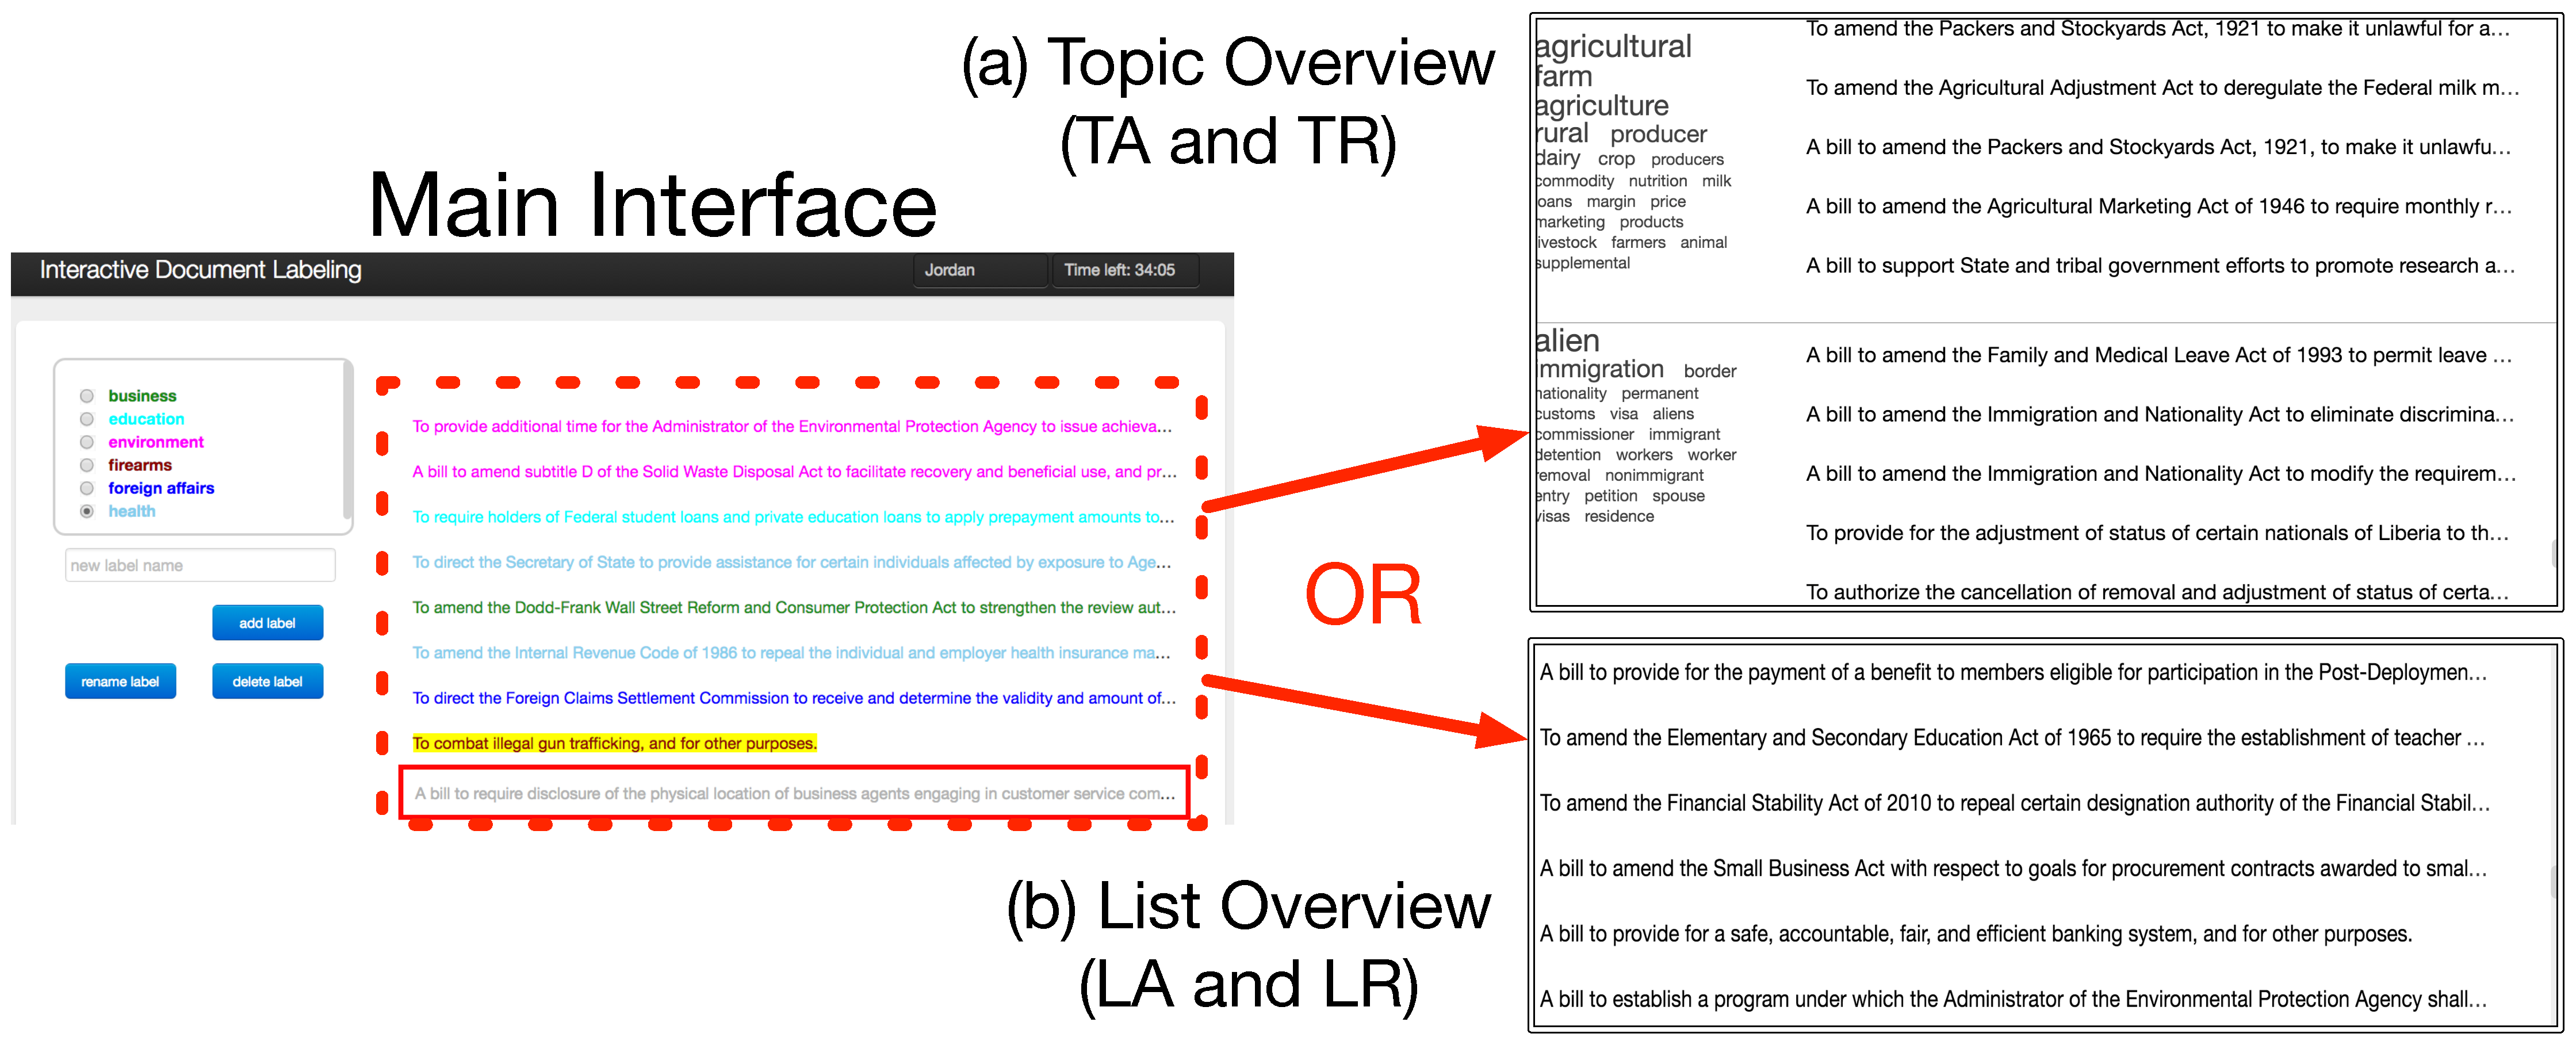
\includegraphics[width=\textwidth]{2016_acl_doclabel/figures/ui_docview}
  \end{center}

	\caption{Our annotation system.  Initially, the user sees lists of
          documents organized in either a list format or grouped into
          topics (only two topics are shown here; users can scroll to
          additional document).  The user can click on a document to
          label it.}
\label{fig:UI-overview}
\end{figure*}



Our goal is to characterize how local and global knowledge can aid
users in annotating a dataset.  This section describes our four
experimental conditions and outlines the user's process for labeling documents.

\subsection{Study Design}
\label{sub:exp_conditions}





The study uses a $2\times2$ between-subjects design, with factors of
document collection \emph{overview} (two levels: topic model or list)
and document \emph{selection} (two levels: active or random). The four
conditions, with the \abr{ta}
condition representing \name{}, are:
\begin{enumerate*}
  \item Topic model and active selection (\abr{ta})
  \item Topic model and random selection (\abr{tr})
  \item List and active selection (\abr{la})
  \item List and random selection (\abr{lr})
\end{enumerate*}

\subsection{Document Collection Overview}\label{sub:UI}



The topic and list overviews offer different overall structure but the
same basic elements for users to create, modify, and apply labels
(Section~\ref{sub:interaction}). The topic overview
(Figure~\ref{fig:UI-overview}a) builds on \newcite{ITM}: for each
topic, the top twenty words are shown alongside twenty document
titles. Topic words ($w$) are sized based on their probability
$\phi_{k,w}$ in the topic $k$ and the documents with the highest
probability of that topic ($\theta_{d,k}$) are shown.  The list
overview, in contrast, presents documents as a simple, randomly
ordered list of titles (Figure~\ref{fig:UI-overview}b). We
display the same number of documents ($20K$, where $K$ is the total
number of topics) in both the topic model and list overviews, but the
list overview obviously provides no topic information.

\subsection{Document Selection}\label{sub:AL}










To provide consistency across the four conditions,  all of the conditions use a
document preference function $U$ to direct the user's attention to a document to label.  For the random selection
conditions, \abr{tr} and \abr{lr}, document selection is random, within a topic or globally.
We expect this to be less useful than active
learning. The document preference functions are:

\noindent
\textbf{\abr{la}}: \abr{la} uses traditional uncertainty sampling:
\begin{equation}\label{eq:AL_UA}
	U_{d}^{\mbox{\abr{la}}} = \h{C}{Y_d},
\end{equation}
 where
$\h{C}{y_d} = -\sum_{i} P(y_i|d)log P(y_i|d)$ is the classifier entropy. Entropy measures how confused (uncertain) classifier $C$ is about its prediction of a document $d$'s label $y$. Intuitively, it prefers documents that most of the labels are likely to be predicted to documents that only one of the labels is highly likely to be chosen.
\noindent
\textbf{\abr{lr}}: \abr{lr}'s approach is the same as \abr{la}'s
except we replace $\h{C}{y_d}$ with a uniform random number:
\begin{equation}\label{eq:AL_UR}
	U_{d}^{\mbox{\abr{lr}}} \sim \mbox{unif}(0,1).
\end{equation}
 In contrast to \abr{la}, which suggests the most uncertain document, \abr{lr} suggests a random document.

\noindent
\textbf{\abr{ta}}: \newcite{Dasgupta-08} argue that clustering should inform
active learning criteria, balancing coverage against classifier accuracy.  We
adapt their method to flat topic models---in contrast to their hierarchical
cluster trees---by creating a composite measure of document uncertainty within a
topic:
\begin{equation}
	U_{d}^{\mbox{\abr{ta}}} = \h{C}{y_d} \theta_{d,k},
\label{eq:AL_TA}
\end{equation}
where $k$ is the prominent topic for document $d$. $U_d^{\mbox{\abr{ta}}}$ prefers
documents that are \emph{representative} of a topic
(i.e., have a high value of
$\theta_{d,k}$ for that topic)
and are informative for the classifier.

\noindent
\textbf{\abr{tr}}: \abr{tr}'s approach is the same as \abr{ta}'s
except we replace $\h{C}{Y_d}$ with a uniformly random number:
\begin{equation}\label{eq:AL_TR}
	U_{d}^{\mbox{\abr{tr}}} = \mbox{unif}(0,1) \theta_{d,k}.
\end{equation}
Similar to \abr{ta}, this prefers
documents that are representative of a topic, but not any particular such document. Incorporating the random component encourages for covering different documents in diverse topics.










   In \abr{la} and \abr{lr}, the preference function directly
chooses a document and directs the user to it. On the other hand, $U^{\abr{TA}}_d$
and $U^{\abr{TR}}_d$ are topic dependent: To avoid the negative and misleading effect of topics, users' attention should be drawn to documents that are representative of a specific topic. Therefore, the factor $\theta_{d,k}$ appears in
both. Thus, they require that a topic be chosen first and then the document
with maximum preference, $U$, within that topic can be chosen. In \abr{tr}, the
topic is chosen randomly. In \abr{ta}, the topic is chosen by
\begin{equation}\label{eq:topic_perference}
    k^{*}=\arg\max_k(\mbox{median}_d(\h{C}{y_d} \theta_{d,k}).
\end{equation}
That is the topic with the maximum median $U$. Median encodes how ``confusing'' a topic is.\footnote{Outliers skew other measures (e.g., max or mean).} Intuitively, $k^{*}$ is the topics that the classifier is confused about its documents' labels.

\subsection{User Labeling Process}\label{sub:interaction}

%\begin{figure*}[t!]
	%\centering
     \begin{figure}[t!]%{0.45\textwidth}
        \centering
        \imagebox{97mm}{\includegraphics[width=\linewidth]{2016_acl_doclabel/figures/UI_labeling}}
  		\caption{Document view: after clicking on a document from the list or topic overview, the user inspects the text and provides a label.  If the classifier has a guess at the label, the user can confirm the guess.}
  		\label{fig:UI-label}
        \end{figure}%
       % \begin{subfigure}{0.03\textwidth}
        %  { \  }
      %\end{subfigure}
      \begin{figure}[t!]%{0.45\textwidth}
        \centering
       	\imagebox{45mm}{\includegraphics[width=\linewidth]{2016_acl_doclabel/figures/ui_doc_highlight}}
      	\caption{After the user has labeled some documents, the system can automatically label other documents and select which documents would be most helpful to annotate next.  In the random selection setting, random documents are selected.}
 		 \label{fig:UI-highlight}
       \end{figure}%  
%\end{figure*}



The user's labeling process is the same in all four conditions. The
\emph{overview} (topic or list) allows users to examine individual
documents (Figure~\ref{fig:UI-overview}). Clicking on a document opens a dialog box
(Figure~\ref{fig:UI-label}) with the text of the document and three
options:
\begin{enumerate*}
  \item Create and assign a new label to the document.
  \item Choose an existing label for the document.
  \item Skip the document.
\end{enumerate*}








Once the user has labeled two documents with different labels, the displayed
documents are replaced based on the preference function (Section~\ref{sub:AL}),
every time the user labels (or updates labels for) a document. In \abr{ta} and
\abr{tr}, each topic's documents are replaced with the top twenty most uncertain
documents. In \abr{la} and \abr{lr}, all documents are updated with the top
$20K$ uncertain documents.\footnote{In all conditions, the number of displayed unlabeled documents is adjusted based on the number of manually labeled documents. i.e. if the user has labeled $n$ documents in topic $k$, $n$ manually labeled documents followed by top $20-n$ uncertain documents will be shown in topic $k$.}

The system also suggests one document to
consider by auto-scrolling to it and drawing a red box around its title
(Figure~\ref{fig:UI-highlight}). The user may ignore that document and click on any other
document. After the user labels ten documents, the classifier runs and assigns
labels to other documents.\footnote{To reduce user confusion, for each existing
  label, only the top 100 documents get a label assigned in the \abr{ui}.} For
classifier-labeled documents, the user can either approve the label or assign a
different label. The process continues until the user is satisfied or a time
runs out (forty minutes in our user study, Section~\ref{sec:user_exp_results}).
We use time to control for the varying difficulty of assigning documents: active
learning will select more difficult documents to annotate, but they may be more
useful; time is a more fair basis of comparison in real-world tasks.